%--------------------
% Packages
% -------------------
%\documentclass[11pt,a4paper]{article}
%\usepackage[utf8x]{inputenc}
%\usepackage[T1]{fontenc}
%\usepackage{gentium}
%\usepackage{mathptmx} % Use Times Font
%\usepackage{svg}
%\usepackage{caption}
%\usepackage{changepage}

%\usepackage[pdftex]{graphicx} % Required for including pictures
%\usepackage[swedish]{babel} % Swedish translations
%\usepackage[pdftex,linkcolor=black,pdfborder={0 0 0}]{hyperref} % Format links for pdf
%\usepackage{calc} % To reset the counter in the document after title page
%\usepackage{enumitem} % Includes lists

%\frenchspacing % No double spacing between sentences
%\linespread{2.0} % Set linespace
%\usepackage[a4paper, lmargin=0.1666\paperwidth, rmargin=0.1666\paperwidth, tmargin=0.1111\paperheight, bmargin=0.1111\paperheight]{geometry} %margins
%\usepackage{parskip}
%\usepackage{amsmath}

%\usepackage[all]{nowidow} % Tries to remove widows
%\usepackage[protrusion=true,expansion=true]{microtype} % Improves typography, load after fontpackage is selected
%\usepackage{tabto}
%\usepackage{apacite}
%\bibliographystyle{apacite}
%\usepackage[inkscapelatex=false]{svg}
%\usepackage{comment}
%\usepackage{lipsum} % Used for inserting dummy 'Lorem ipsum' text into the template


%-----------------------
% Set pdf information and add title, fill in the fields
%-----------------------

%%%----------SETUP----------%%%

\documentclass[11pt, titlepage]{article}



% MACSS packages:

\usepackage{lmodern}
\usepackage[margin=1.25in, headheight=14pt]{geometry}
\usepackage{setspace}
    \onehalfspacing
\usepackage[dvipsnames]{xcolor}
\usepackage{tabularray}
\usepackage{nameref}
\usepackage{fancyhdr}
\usepackage[style=apa]{biblatex}
    \addbibresource{references_test.bib}
\usepackage[colorlinks=true, 
            allcolors=RoyalBlue,
            citecolor=.]{hyperref} 
%\usepackage{graphicx}
% Anita's packages:

\usepackage{caption}
\usepackage[pdftex]{graphicx} % Required for including pictures
\usepackage[inkscapelatex=false]{svg}
\usepackage{comment}
\usepackage{changepage}
%%  Set biographic information for the title page and document

\newcommand{\thesistitle}{\#2024election: An Exploratory Analysis of Politicultural Communities on TikTok}
\newcommand{\thesisauthor}{Anita Sun}
\newcommand{\graddate}{June 2026}
\newcommand{\facultyadvisor}{Dr. David Peterson}
\newcommand{\preceptor}{Dr. Henry Dambanemuya}
\newcommand{\keywords}{Key1; Key2; Key3...}

%% Set PDF metadata
\hypersetup{
  pdfauthor={\thesisauthor \ Copyright \textcopyright \number\year},
  pdftitle={\thesistitle},
  pdfsubject={MACSS MA Thesis},
  pdfkeywords={\keywords},
  pdfborder={0 0 0}
}

%% set up header footer style
\pagestyle{fancy}
\fancyhead{}
\fancyhead[R]{\thesisauthor}
\fancyfoot{}
\fancyfoot[C]{\thepage}




\begin{document}


\begin{titlepage}
    %% Do not edit the titlepage section. Make any changes above
    \begin{center}
        \vspace*{-0.45in}
        
\includegraphics[height = 1.5in]{viz/Shield.png}\\
	\vspace{0.1in}
        \Large{\uppercase{The University of Chicago}}\\
	\vspace{0.8in}
	\LARGE{\textsc{\thesistitle\\}}
	\vspace{0.8in}
	\normalsize{By}\\
	\Large{\thesisauthor\\
	\vspace{0.5in}
	\graddate\\}
        \vspace{0.8in}
	\Large{A paper submitted in partial fulfillment of the requirements for \\
	the Master of Arts degree in the Master of Arts in\\
        Computational Social Science}
        \vspace*{\fill}		
    \end{center}
    \Large{Faculty Advisor: \facultyadvisor \\
    Preceptor: \preceptor\\}
    \vspace*{-0.45in}
\end{titlepage}

\section*{Acknowledgments}

I would like to thank Dr. David Peterson, Dr. Jun Sun, and Peter Zhang, M.A., for their insight and guidance. I could not have completed this thesis without your support.

{\color{Gray}\noindent\hrulefill}

\section*{Abstract}

\bigskip
\noindent\textbf{Keywords:} \keywords

{\color{Gray}\noindent\hrulefill}

\section{Introduction}
On June 7th, 2024, electric pop music artist Charli XCX released her hit album BRAT, which received wide acclaim and garnered huge commercial success. Later that summer, then-Vice President Kamala Harris announced the beginning of her presidential campaign for the upcoming 2024 U.S. Presidential Election. The two seemingly unrelated events would come to intertwine on the social media app and platform TikTok, as a strange remix of Charli XCX’s song Apple incorporating an audio clip of Harris speaking at a press conference exploded in popularity \parencite{clarke-billings_what_2024}.\footnote{As of writing, the most-liked TikTok post playing this “Coconut” remix of Charli XCX’s "Apple" has over 6.7 million views and over 1.2 million likes total.}  In order for this bizarre combination of politics and music to skyrocket into virality, there needed to be some overlap in the groups of TikTok users who knew of Charli XCX and users who knew of former Vice President Kamala Harris. The question remains, how much overlap was there between those two groups? For this research proposal, I explore TikTok to ask if partisan preference is associated with difference in culture and entertainment preferences on the platform. This can be broken down into two main research questions:

RQ 1: Of the TikTok users who followed official TikTok campaign accounts, what are the topics of those users’ reposted TikTok posts as represented by each post's hashtags and caption information?

RQ 2: Of the TikTok users who followed official TikTok campaign accounts, what are the bipartite network structures of co-occurring hashtags in the TikTok posts that were reposted by those followers, and how do they compare with each other?


\section{Literature Review}

\subsection{Politics, Attitudes, and Preferences}

It is well documented in previous literature that political attitudes and preferences permeate deeply and widely into individual's social lives and identities. Politicultural sorting, or the fragmentation of American cultures along political affiliation, is demonstrated in one study that uses National Consumer Survey data to show liberal and conservative ideology each encompass multiple cultural archetypes \parencite{rogers_politicultural_2022}. Another study finds that liberals and conservatives from the same college campus spend their time differently in small but robust ways, physically occupying separate geographic spaces \parencite{talaifar_lifestyle_2025}. This effect was more strongly observed for individuals' leisure time; furthermore, there is a difference in the way that Democrats and Republicans perceive content on social media platforms \parencite{talaifar_lifestyle_2025} \parencite{mcclain_how_2024}.  Not only is this cultural and behavioral partisanship exhibited by individuals, but individuals can also recognize this partisanship in others. Studies have shown that individuals can correctly identify others' political affiliations using non-political cues and information, such as one's preferences in music or clothing \parencite{deichert_partisan_2019} \parencite{lee_how_2021}. Perhaps more importantly, individuals use these inferences on political affiliation to decide whom to interact with, which can further encourage in-group interaction and cause more cleavage between parties \parencite{deichert_partisan_2019} \parencite{lee_how_2021}. 

The politicultural divide extends to social media preferences and behaviors as well. One study shows that political polarization extends to brand-preference polarization on Twitter following the 2016 and 2020 Presidential election \parencite{schoenmueller_frontiers_2023}. Individuals who engage in partisan spheres on social media exhibit different patterns of interaction compared to non-partisans \parencite{mamakos_social_2023}; user behavior on social media also varies by party, even when the topic at hand is not inherently related to politics \parencite{pendse_role_2025} \parencite{essig_partisan_2024}. Opinions and perception of social media platforms vary by party, TikTok included \parencite{mcclain_how_2024}. 
This difference in culture and behaviors along partisan lines, on social media and otherwise, along with partisan differences in perceptions of TikTok, suggest that TikTok usage is likely to vary by political preference.  With recent shifts in American political landscape, such as the increased influence of far-right politics and affective polarization \parencite{brown_far_2023}\parencite{polacko_rightward_2022}, it is likely that this politicultural divide is also shifting. TikTok may be a platform with unique insight to analyze this shift, given its recent popularity and increased political relevance with American youth \parencite{mcclain_how_2024}. However, literature surrounding TikTok is currently sparse, and more disconcertingly, easily outdated, due to the temporal and rapidly-evolving structure of the platform.

\subsection{TikTok and Its Eccentricities}

One particularity of TikTok as a social media platform is how unrepresentative its users are of the broader American public; a prevalent feature of the app is the extent to which it appeals to younger users. This particularism flows bidirectionally; TikTok has shown to be more politically influential for young adults than other social media platforms, and there is also a disproportionately larger share of younger users on TikTok than other age groups in comparison to other social media platforms \parencite{karimi_scrolling_2023} \parencite{mcclain_how_2024}. Not only is the app more widely used by youth, there is evidence that TikTok usership is predictive of higher rates of civic engagement and in-person activism efforts \parencite{karimi_scrolling_2023} \parencite{oden_kids_2023}. Adolescents and young adults also seem to be more proficient at communicating on TikTok, leveraging their knowledge of algorithmic patterns and “algospeak” to bypass content moderation of certain keywords or topics \parencite{steen_you_2023}. This new form of communication contrasts with the linguistic structure of traditional media outlets such as news stations and journals, and as such there is a clear generational divide on the app.

With this clear emphasis on rapidly evolving slang and equally temporal trends, it is no mystery why much of the extant literature on TikTok and politics surrounds youth organizing and the way TikTok’s communication differs from other social media platforms \parencite{abbas_tiktok_2022} \parencite{cervi_playful_2023} \parencite{hindarto_tiktok_2022}. However, the shape of the overall political landscape remains largely unclear; though some studies report a liberal or left-biased slant for the overall spread of content on TikTok and its user demographic \parencite{mcclain_how_2024} \parencite{karimi_scrolling_2023}, other studies claim that in terms of total output, right-wing political content prevails \parencite{widholm_right-wing_2024} \parencite{medina_serrano_dancing_2020}. As the platform grew in popularity, politicians and political bases began to adopt TikTok as a means of reaching voters and constituents \parencite{moir_use_2023}, with interesting implications as to how posts such as “thirst traps” and various “TikTok style edits” can influence the perception of politicians by the public \parencite{munger_thirst_2025}, highlighting the salience of structure and format in political communication on TikTok.

\subsection{The Gap In Literature}

Past scholarship has utilized these unique structures of communication on TikTok to examine interactions not found on other social media platforms. Its growing popularity has also enabled scale-up of research studies that would not have been possible just years prior. For example, Medina Serrano et al. \parencite*{medina_serrano_dancing_2020} use a web crawler to collect videos, which are then analyzed using Microsoft’s Azure Face API. Another group of researchers trains a neural network to classify TikTok videos filmed in second person view and non-second person points of view in order to compare engagement differences between the two types of videos \cite{cheng_like_2024} . Other computational researchers take advantage of TikTok’s Research Tools API, including one such group of researchers who analyzed political discourse surrounding the 2024 election prior to former President Joe Biden’s withdrawal \parencite{pinto_tracking_2024}. Another study makes use of Amazon’s Mechanical Turk to administer a large-scale survey, highlighting another computational method that deviates from what otherwise has been a predominantly qualitative body of work about TikTok \parencite{karimi_scrolling_2023} \parencite{hindarto_tiktok_2022} \parencite{kanthawala_its_2022}.

My research project is aimed at filling the gap between the study of politics on TikTok and politics in relation to other facets of social life. Shi et al. \parencite*{shi_millions_2017} conducted a conceptually similar study by analyzing the relationship between political affiliation and interest in science through Amazon book purchase history, connecting political affiliation to other aspects of individual identity. We have ample literature on the structure of the platform, the rhetorical and linguistic strategies employed in political communication, and of TikTok’s unique relationship with youth; what remains unknown is how the bi-partite cultural networks of TikTok users differ in their structure and contents. In my next section, I will take advantage of TikTok’s platform structure in building a dataset to examine this very question.

\section{Data and Methods}

\begin{figure}[t]
\includesvg[scale=0.8]{viz/Data_Structure_Cohash.svg}
\captionof{figure}{Dataset structure, using @kamalahq as the example campaign TikTok account.}
\label{data_tree}
\end{figure}

\subsection{Data Structure}

Using the TikTok API, I queried and obtained all the data required for analysis. The dataset for this study branches out in a tree-like structure, shown in Figure \ref{data_tree}. I first identified official platform-verified TikTok campaign accounts for Harris and Trump, which are @kamalahq and @teamtrump, respectively. I then collected the usernames of the accounts that most recently followed each campaign account as of December 23, 2025. The ambiguity in time range is a result of the forced backwards pagination design in the API, which allows me to access only the most recently added followers. I was able to collect 462 follower usernames for @kamalahq and 511 follower usernames for @teamtrump for a total of 973 TikTok users. These two groups of users are disjoint; each user in this dataset follows only one of the two campaign accounts. The difference in numbers is due to various types of missingness or redaction in the data collection process, which includes deleted accounts, underage accounts, and private accounts. As of the time of writing, the TikTok Research Tools API documentation lists the aforementioned reasons as potential causes of missingness, but also notes that other unaccounted factors can cause missingness. Therefore, the difference in size between the two groups of followers could be caused by systemic or random differences.

After constructing the dataset of campaign account public followers, I scraped the metadata of each reposted TikTok video from each of the 973 users, resulting in 1,298,363 Harris follower reposts and 402,861 Trump follower reposts. The video metadata I use in my analysis are the video descriptions, which is the text shown at the bottom of a video, and the hashtags, which are a list of hashtags found within the video description. Though hashtags are contained within video descriptions, I use both hashtags and video descriptions in my analysis because some methods, like network modeling, are better suited to hashtags, whereas other methods, such as document embeddings, are better suited to video description text.
\begin{comment}
\begin{figure}
\begin{adjustwidth}{-2cm}{-2cm} % Adjust margins: left and right
    \begin{minipage}{\linewidth}
        \centering
        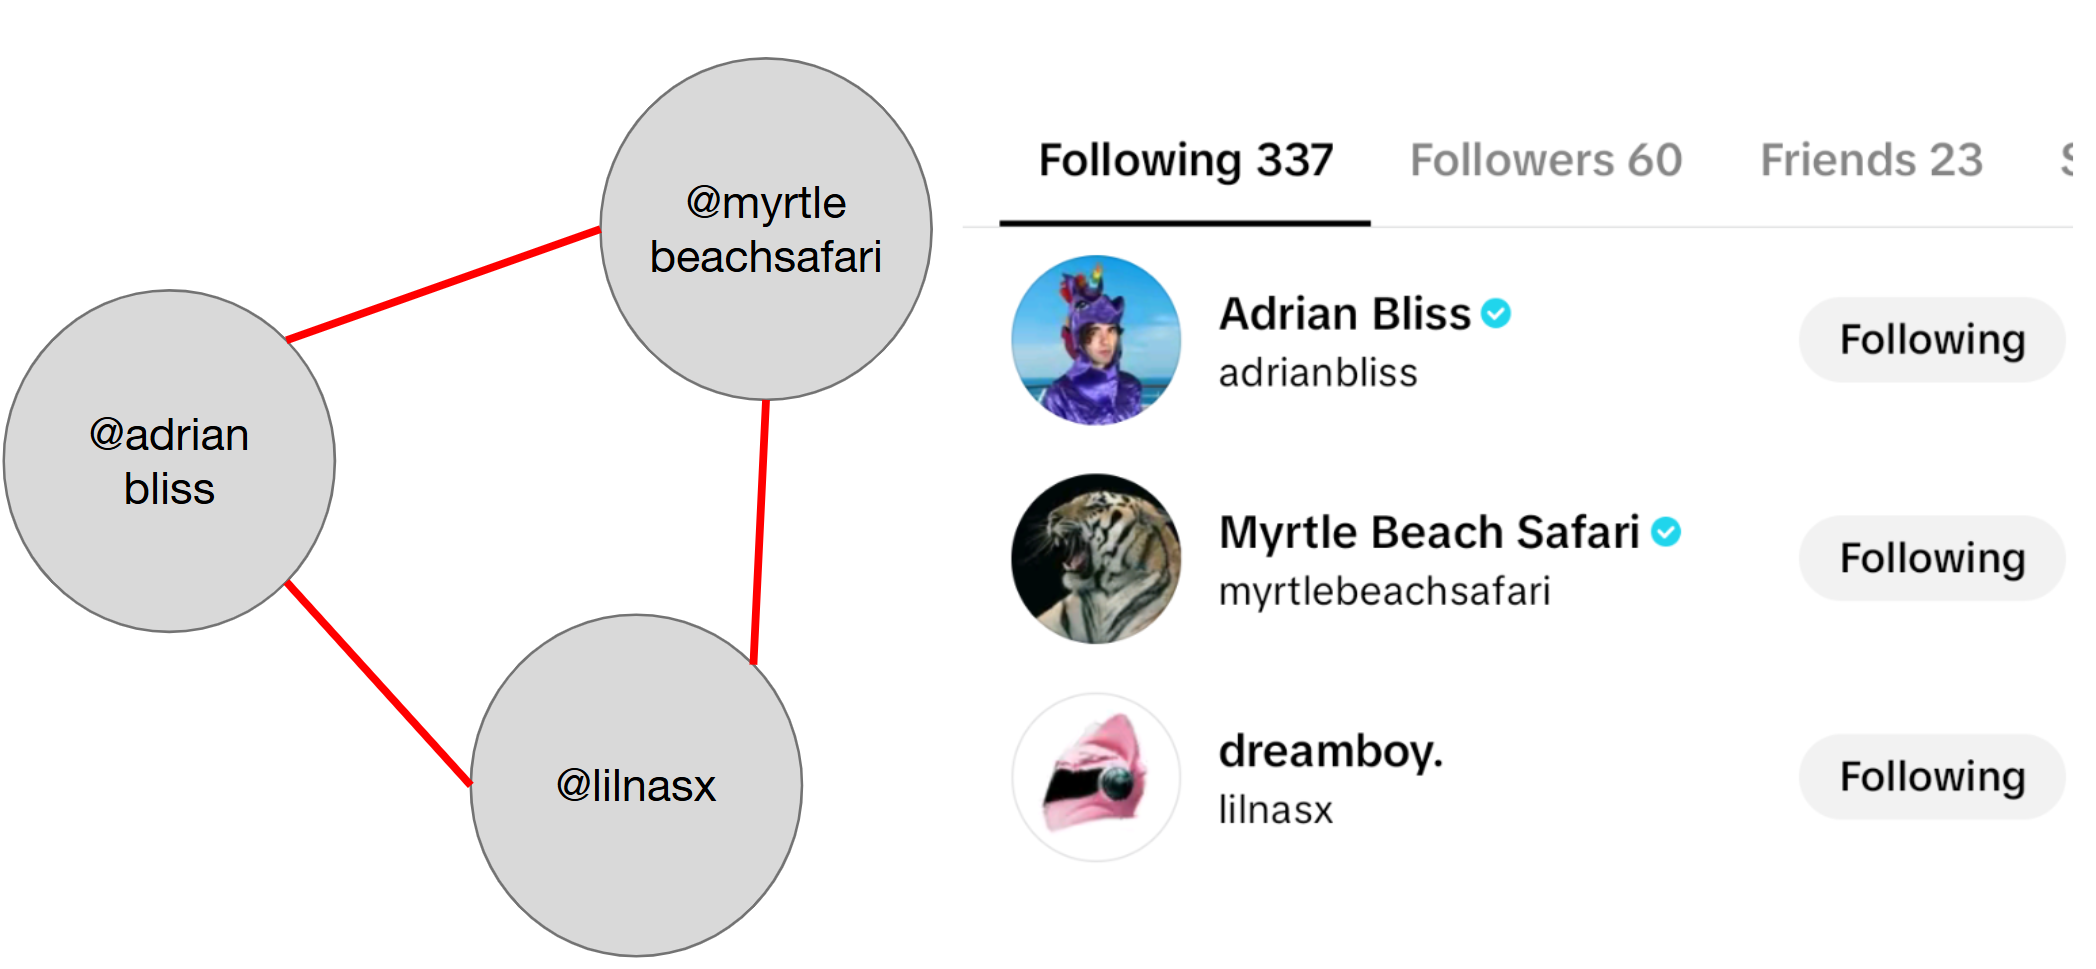
\includegraphics[width=\linewidth]{viz/cofollowing_net.png}
        \captionsetup{width=0.9\linewidth, justification=centering} 
        \captionof{figure}{A scaled down example of constructing a co-follow network, where each follower constitutes an edge between any two users they follow}
    \end{minipage}
\end{adjustwidth}
\end{figure}
\end{comment}

\begin{figure}[t]
\begin{adjustwidth}{-2cm}{-2cm} % Adjust margins: left and right
    \begin{minipage}{\linewidth}
        \centering
        %\label{cohash_ex}
        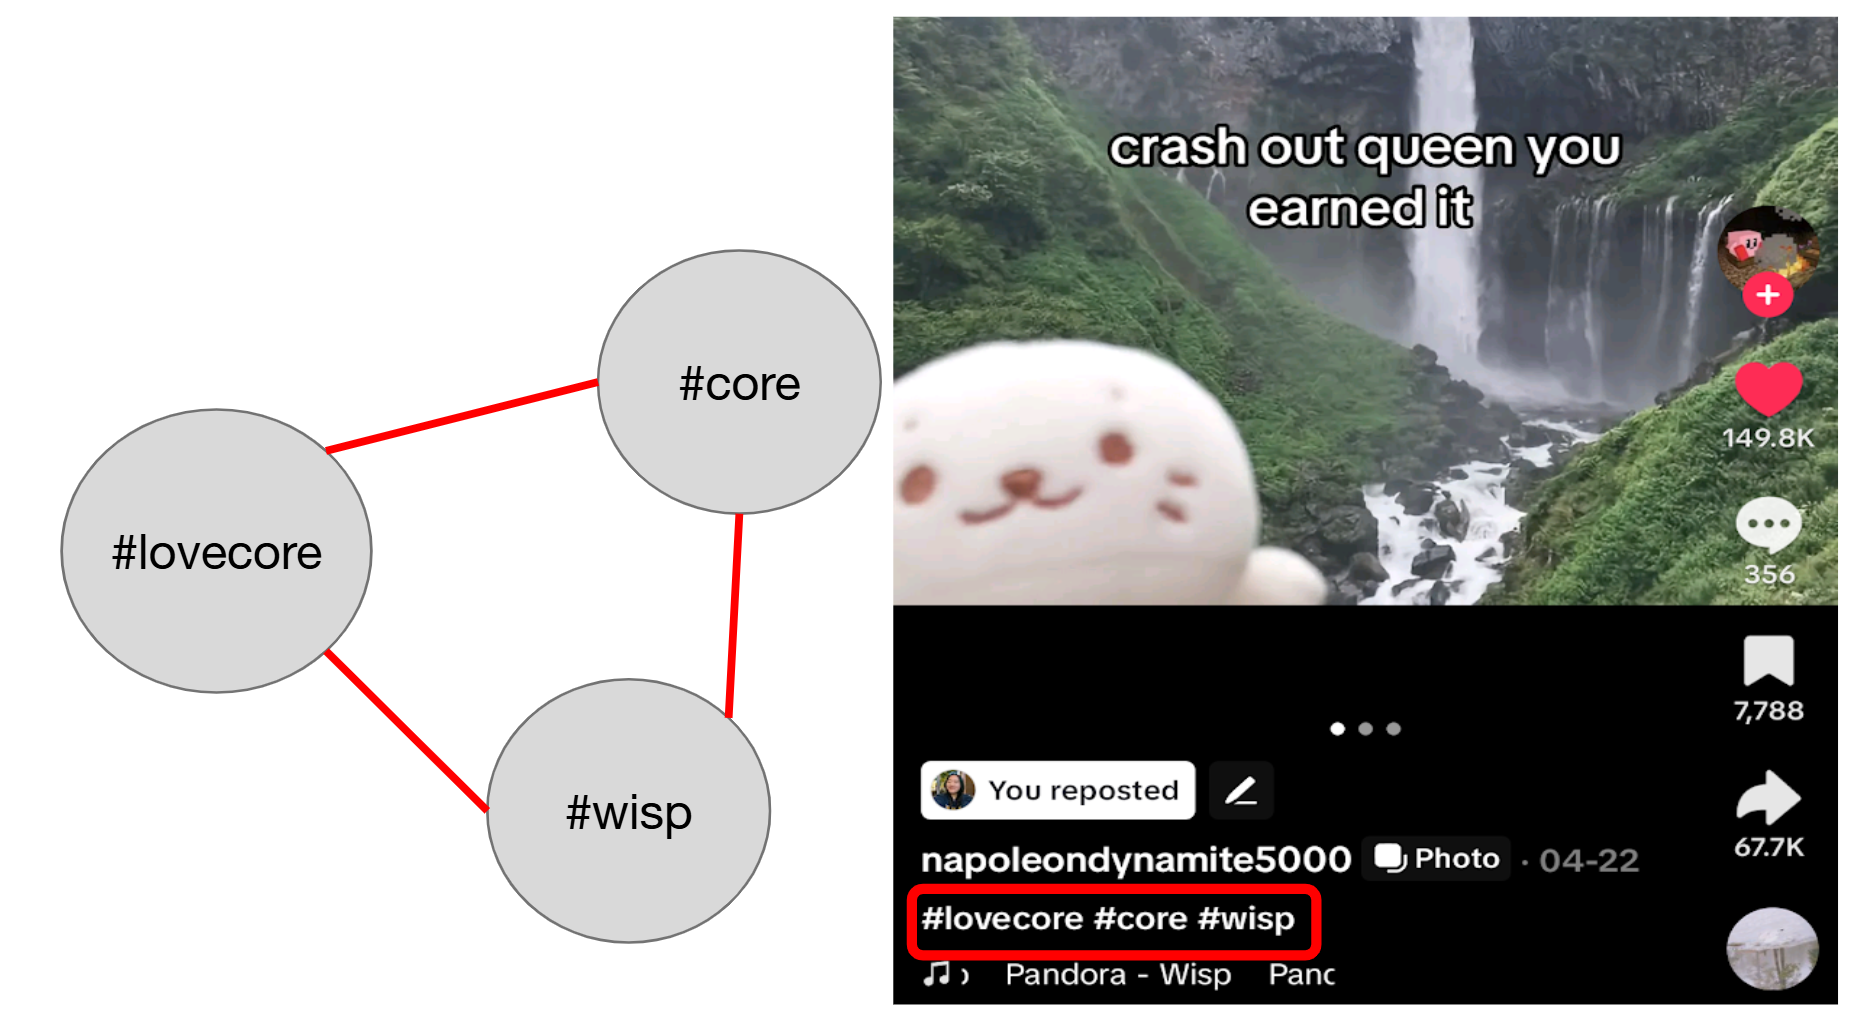
\includegraphics[width=\linewidth]{viz/cohashtag_net.png}
        %\label{cohash_ex}
        \captionsetup{width=0.9\linewidth, justification=centering} 
        \captionof{figure}{A scaled down example of constructing the co-hashtag network, where each TikTok repost constitutes an edge between any two hashtags in the video description.}
        \label{cohash_ex}
    \end{minipage}
\end{adjustwidth}
\end{figure}

\subsection{Methods}

Using this dataset, I perform three different methods of analysis. The first two methods focus on substantive analysis of TikTok videos, whereas the third method is focused on a structural analysis. The first method I use is itemset mining, drawing inspiration again from Shi et al. \parencite*{shi_millions_2017}, where researchers take advantage of Amazon's suggested co-purchase itemsets regarding online book sales. Itemset mining, or association rule mining, is suited to analyzing frequently co-occurring items. Due to the large scale of my dataset, I use a Frequent Pattern Growth (FP-Growth) algorithm as designed by Han et al. \parencite*{han_mining_2000} to reduce computational costs. I apply FP-Growth itemset mining to the TikTok videos reposted by the followers of @kamalahq and @teamtrump by analyzing each video as a set of co-occurring hashtags. One benefit of itemset mining is that it is directional and therefore distinguishes between symmetrically and asymmetrically implicative relationships amongst items in a set. For example, the frequent itemset [\#billieeilish $\rightarrow$ \#edit] demonstrates that in posts where \#billieeilish is tagged, \#edit is also frequently tagged, but it does not imply that \#billieeilish is frequently tagged in posts containing \#edit. 

%The first layer concerns the official presidential campaign TikTok posts themselves. I will conduct sentiment and topic analysis on this core corpus of videos; each TikTok post will constitute a document in the corpus, and each document will consist of the caption text and the auto-transcript text appended together. From here, I will use apply RoBERTa to the corpus to determine the primary sentiments in these TikTok posts for each candidate. Additionally, I will use BERTopic to cluster and define topics within each candidate’s posts to examine the primary subject matters of the campaign effort. Upon a precursory glance at these campaign TikTok videos, it seems that there are two broad categories in campaign strategy: promoting oneself and one’s policies as the ideal candidate for America, or drawing attention to perceived flaws and deficiencies in the opponent’s campaign. Understanding the sentiment and topic distributions in candidates' campaigns will give a quantitative representation of each candidate's campaign strategy. Though this is not a direct representation of the types of content that campaign account followers are interested in, it can give insight as to what the campaign managers perceive to be the interests and cultural knowledge of the follower base.
 For my second method of analysis I will construct a hashtag co-occurrence network to see how ideas within these partisan spaces relate to each other. In this weighted network, each node represents a hashtag, and each edge between two hashtags represents the number of times the two hashtags co-occur in a TikTok repost. For an example, refer to Figure \ref{cohash_ex}. Using network analysis measures such as clustering coefficient, diameter, average shortest path, I compare the two networks to each other in shape and size. I also examine nodes of interest and prestige using centrality measures such as closeness centrality, betweenness centrality, and eigenvector centrality to identify hashtags that may be indicative or representative of popular topics. The mixture of network-level measures and hashtag-level measures gives both structural and substantive understanding of the corpus and helps to connect the semantic meanings of hashtags themselves to their relative positions in the network. 

Finally, for my third method of analysis, I turn towards interpreting the contents of TikTok posts that were reposted by followers of @kamalahq and @teamtrump. Using the video description text of TikTok reposts as documents, I fit a mixed deep-learning and unsupervised learning BERTopic clustering pipeline for each candidate's followers' text \parencite{grootendorst_bertopic_2022}. However, it would be too computationally expensive to fit the topic model on the entirety of the text. Instead, I perform a grid search over bootstrap samples and compare each iteration's out-of-sample silhouette score, pair-wise topic cosine similarity, and number of topics. I select the iteration with the highest silhouette score that contains between 15 and 30 topics to qualitatively interpret the contents of the corpus. Using the distributions of silhouette scores and pair-wise topic cosine similarity, I compare the two follower bases' discursive structure. By examining the resulting topic clusters, I can infer intra-topic and inter-topic heterogeneity and the relative distances between topic clusters. I evaluate the quality of topics by using silhouette score, which broadly measures the distance of documents to their own topic's centroid against the distance to centroids of other topics. I further examine the distribution of topics by comparing average pair-wise topic cosine similarity in a statistical test, which will give insight to the spread and diversity of topics. 
%be the co-following network of public account users who also follow official campaign TikTok accounts. For each public follower of an official campaign account, I will gather all a list of all accounts that the user follows. This data allows me to graph a co-following network between followers of Harris's campaign and followers of Trump's campaign. From here, I will analyze measures of betweenness and centrality for each campaign pool separately and in conjunction. This analysis will also reveal which public accounts are more likely to be followed by Trump followers and which are more likely to be followed by Harris supporters, which lends itself to more granular investigation of that page's content.


These analyses all help to fill out the substantive and structural landscape of the politicultural divide on TikTok. While itemset mining can identify crucial hashtag tokens and relationships, network analysis can provide insight into larger community structure. Finally, topic modeling provides a corpus-level substantive summary of the corpus contents. Using combined methods create a comprehensive picture of the politicultural landscape by providing insight to different facets of socialization: the stuffing, the scaffolding, and the sinew.
%I will examine the profiles of users who follow official campaign TikTok accounts. From the profiles of public user accounts, I will collect the TikTok post information of all reposted TikTok videos within the valid time frame defined earlier. This information would include the timestamp, caption text, hashtags, and music. In my last layer of analysis, I will again conduct topic analysis using BERTopic to cluster TikTok reposts, defining once again each document as the caption text appended to the auto-transcript text. Using this analysis, I can begin to explore how reposted TikTok videos differ between the two different political bases. From this hashtag data, I can also create a co-hashtag network to see which hashtags are more likely to be reposted by Harris followers and which are more likely to be reposted by Trump followers.

\begin{figure}
\begin{adjustwidth}{-2cm}{-2cm} % Adjust margins: left and right
    \begin{minipage}{\linewidth}
        \centering
        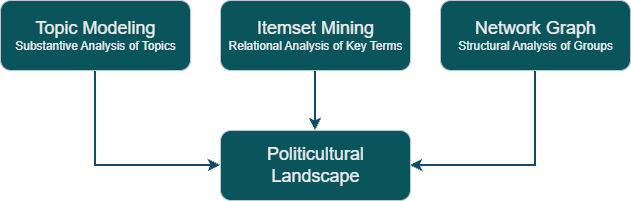
\includegraphics[width=0.9\linewidth]{viz/Design_flow.png}
        \captionsetup{width=0.9\linewidth, justification=centering} 
        \captionof{figure}{The contributions of the three different analytical methods towards one main goal.}
    \end{minipage}
\end{adjustwidth}
\end{figure}

\subsection{Concerns and Critiques}

The biggest weakness of this analysis is the non-random and non-representative data. The follower dataset that I gathered is not a random sample of all of the followers of @kamalahq and @teamtrump. Furthermore, the followers collected are recent followers, meaning they followed the campaign accounts roughly a year after the end of the election. This may confound some of the results and reduce generalizability. %My biggest concern as of now is that my proposed dataset is contingent upon the functionality of the TikTok Research API, and the access to the API is not guaranteed. If I were to be denied access to the API, then I would have two other options for data collection.

There is also the theoretical concern of how politics and political attitudes are framed. Insofar as the Democratic Party espouses liberal politics and the Republican Party is considered conservative, we might also extend these labels to the users who follow the accounts of the party leaders with little doubt; however, that would be an oversight of the shifting political spectrum of American politics. Affective polarization has consolidated partisan division for both the public and for elites \parencite{iyengar_origins_2019} \parencite{flamino_political_2023}, but public opinion itself can be cued by party policies \parencite{yeung_self-reported_2025}.  Thus, the true relationship between an individual's ideology and party identity is difficult to assess, and furthermore neither extractable from my data nor relevant to the research question. For the purposes of this thesis, I reduce political attitudes to partisanship, wherever these parties may fall on a political spectrum. I will not attempt to dissect the ideologies of these parties and relate them to any findings about behavior on TikTok; I will make no claims of the liberalism or conservatism, left wing or right wing ideologies of the two major political parties in the U.S., but rather allow parties to exist as their own entity and observe them as a generative collective with their own cultures and interests.

Finally, there is the issue of interpreting a user following a campaign TikTok account as support or preference for the candidate's party. There is the possibility that pruning users that follow both candidates' accounts will actually remove the users who are most politically engaged and therefore most strongly hold their political attitudes, which may or may not be aligned with a political party. It also not completely certain that individuals who only follow one of the two major party candidates support that party and that candidate. Short of combing through all of the followers' profiles, following is a more consistent behavioral heuristic compared to commenting, liking, and reposting. The latter options are sporadic behaviors that need to be evaluated in their volume and frequency; with commenting, the textual data would need to be analyzed, which can be difficult with brief comments or comments that reference pop culture. By drawing upon the pool of followers, we can create a well-defined sample that isn't subject to inconsistent behavior.

\section{Results}

\subsection{Frequent Itemset Mining}
\label{frequent_itemset_mining}
\begin{figure}[h]
\begin{adjustwidth}{-2cm}{-2cm} % Adjust margins: left and right
    \begin{minipage}{\linewidth}
        \centering
        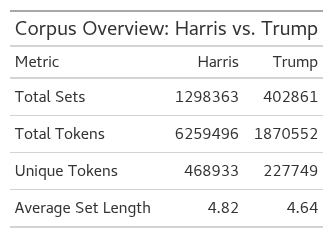
\includegraphics[width=0.4\linewidth]{viz/great_table_itemset_stats.png}
        \captionsetup{width=0.9\linewidth, justification=centering} 
        \captionof{figure}{Descriptive statistics of the hashtag corpus used for frequent itemset mining. In this table, the word "set" refers to one TikTok post containing any number of hashtags. Note that there are nearly three times as many reposts from Harris followers compared to reposts from Trump followers.}
        \label{great_table_itemset_stats}
    \end{minipage}
\end{adjustwidth}
\end{figure}

Upon first glance, it appears that Harris’s followers have a richer and larger corpus of TikTok repost hashtags. Figure \ref{great_table_itemset_stats} shows preliminary hashtag overview. Despite there being fewer Harris followers in the dataset, there are roughly three times as many TikTok videos reposted by the Harris followers compared to Trump followers. The Harris follower corpus additionally has more than twice as many unique hashtag tokens compared to the Trump follower corpus, and each repost on average contains more hashtags. Harris followers repost and thereby endorse TikTok content more frequently, and the content they repost are also richer in hashtags. 

There are several measures to consider when evaluating the validity and insightfulness of association rules. The first is confidence, which is defined as:

\begin{center}$conf(I \rightarrow j)= P( j | I ) =  \frac{P(I,j)}{P(I)}   =  support(I \cap j)/support(I)$
\end{center}

which measures the extent to which the antecedent item, $I$, implies the consequent item, $j$. If the confidence of the association rule [\#billieeilish $\rightarrow$ \#edit] is 0.80, then 80\% of all posts containing \#billieeilish also contain \#edit. This is a general measure of how strongly associated these two items are. Another measure to consider is lift, which is defined as follows:
\begin{center}
$lift(I \rightarrow j) =  \frac{conf(I \rightarrow j)}{(P(j)}$
\end{center}
which is the ratio that measures the magnitude to which $I$ amplifies or “lifts” the likelihood of $j$. If the lift of [\#billieeilish $\rightarrow$ \#edit] is 2.5, then \#edit is 2.5 times as likely to be tagged if \#billieeilish is also tagged.
\begin{figure}
\begin{adjustwidth}{-2cm}{-2cm}
    \begin{minipage}{\linewidth}
        \centering
        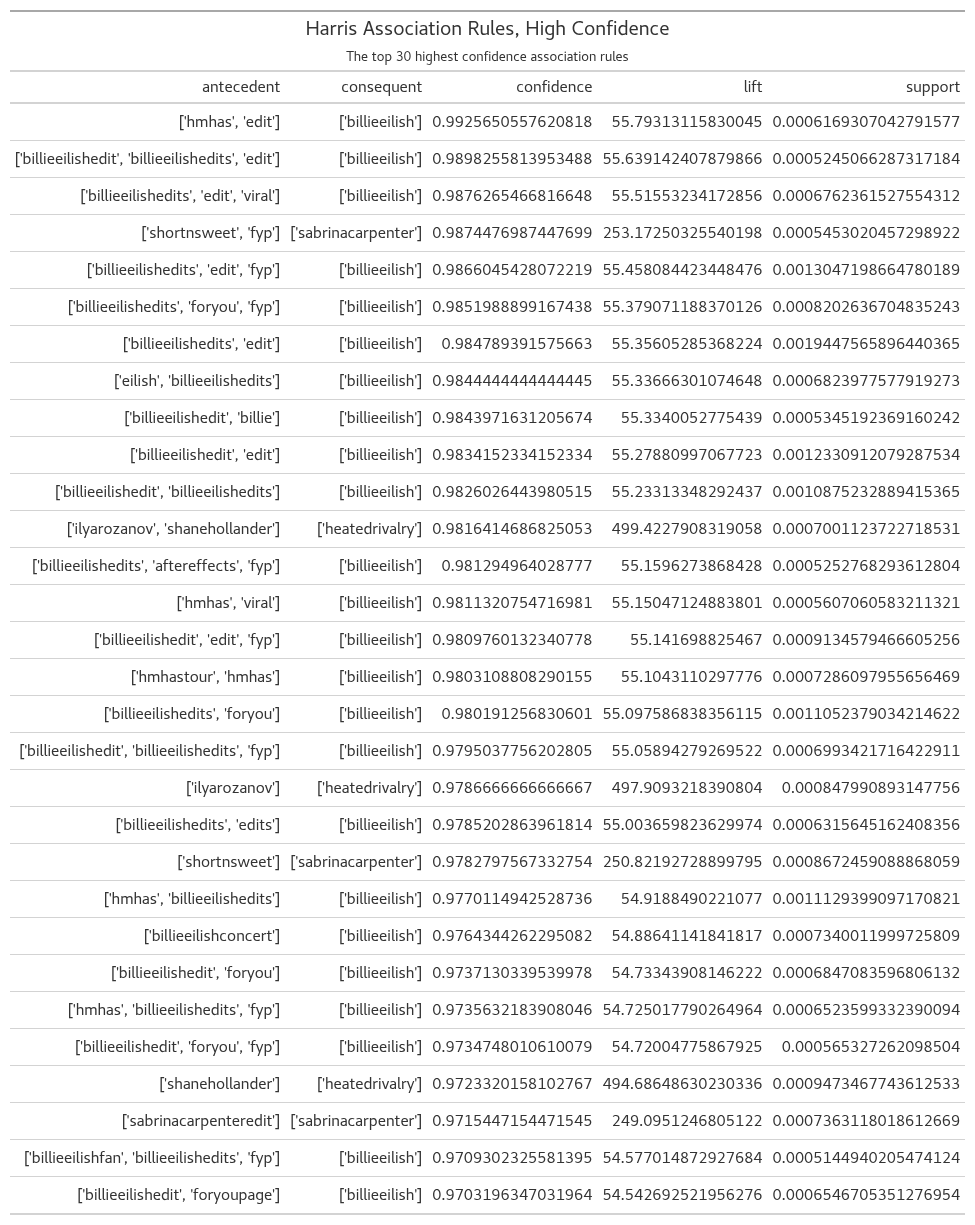
\includegraphics[height=7in]{viz/gt_kamala_association_rules.png}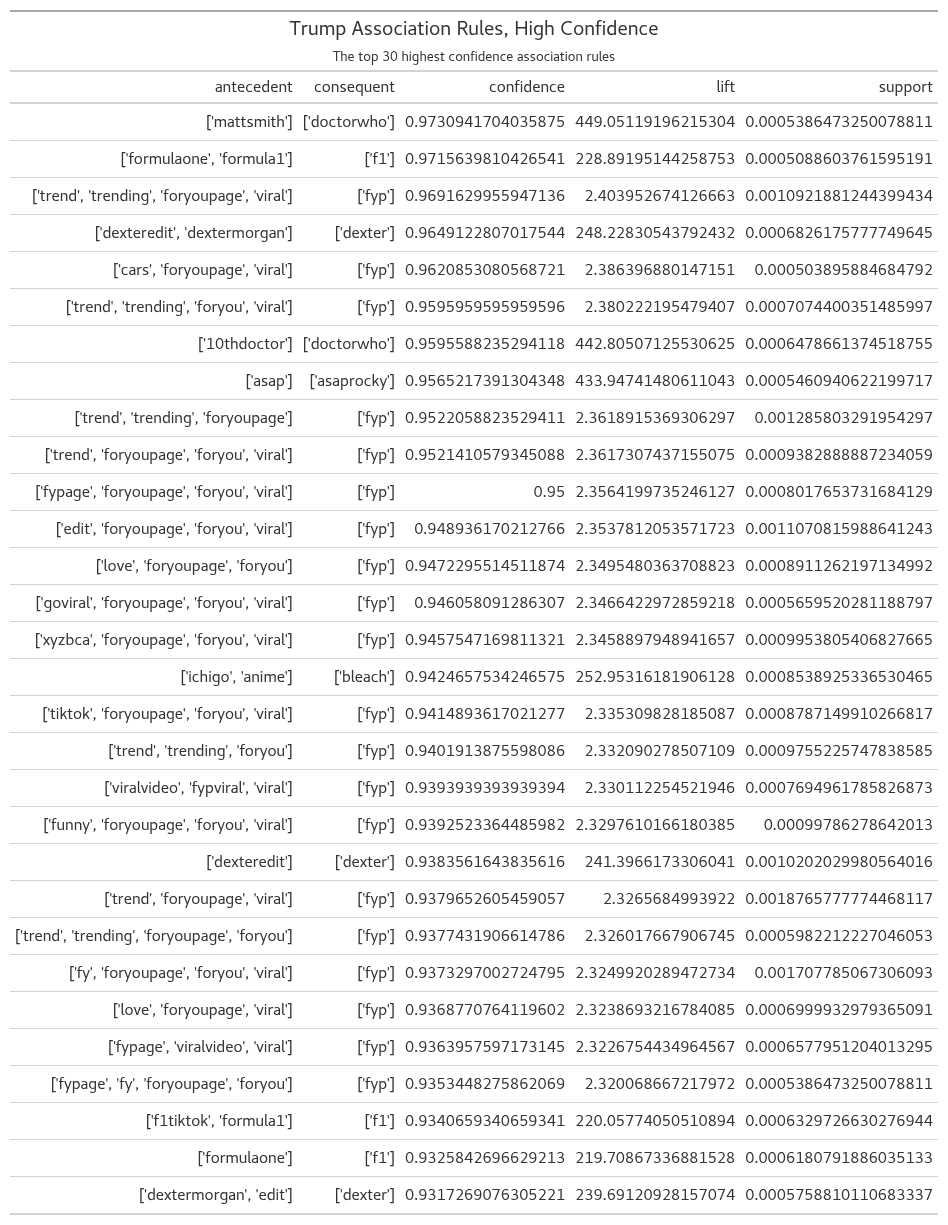
\includegraphics[height=7in]{viz/gt_trump_association_rules.png}
        \captionsetup{width=0.9\linewidth, justification=centering} 
        \captionof{figure}{The highest confidence association rules for Harris and Trump followers, depicted on the left and right, respectively.}
        \label{high_confidence_rule}
    \end{minipage}
\end{adjustwidth}
\end{figure}

Figure \ref{high_confidence_rule} displays the highest confidence association rules found after FP-Growth itemset mining. This offers a glimpse into the discourse patterns for each candidate's follower group. Pop music artist Billie Eilish and her sophomore album, \textit{HIT ME HARD AND SOFT,} abbreviated as "hmhas", dominate the high confidence association rules in the Harris hashtags. Eilish is joined on this list by her peer Sabrina Carpenter, another pop music artist, whose album \textit{Short n' Sweet} won the 2025 Grammy Award for \textit{Album of the Year} and \textit{Best Pop Vocal Album} \parencite{frazier_2025_2025}. Ilya Rozanov and Shane Hollander, fictional hockey players from the novel and recently adapted television show, \textit{Heated Rivalry,} also make appearances in high confidence association rules.

The patterns found in high confidence association rules in Trump hashtags are not quite as concrete and specific. The majority of the association rules are connected to the hashtag '\#fyp', which is an abbreviation of "For You Page." The For You Page on TikTok is akin to an explore or discovery page that has been attuned to the user's preferences and engagement patterns. The hashtag '\#fyp' therefore does not provide information about the contents of the TikTok post but rather indicates the post creator's desire to increase the chances of the post being shown on other users' For You Pages. Variations of '\#fyp' include tags such as '\#foryou', '\#foryoupage', '\#fypage', and more. Other tags such as '\#trend' and '\#viral' are used to increase a post's visibility and are functionally similar to '\#fyp'. I will refer to these hashtags as \textit{engagement hacking hashtags}. Aside from engagement hacking hashtags, there are a few references to media and entertainment in the high confidence association rules. For example, the hashtag '\#asap' generally refers to rapper A\$AP Rocky rather than "as soon as possible." The fiction book series \textit{Dexter} and its multiple television adaptations are also featured, as well as the science fiction television show \textit{Doctor Who}.\footnote{The English actor Matt Smith portrays the character of the 11th Doctor in the television series. Curiously, the 10th Doctor also makes an appearance in the high confidence association rules, but the actor who portrays him, David Tennant, does not.}

\begin{figure}[h]
\begin{adjustwidth}{-2cm}{-2cm}
    \begin{minipage}{\linewidth}
        \centering
        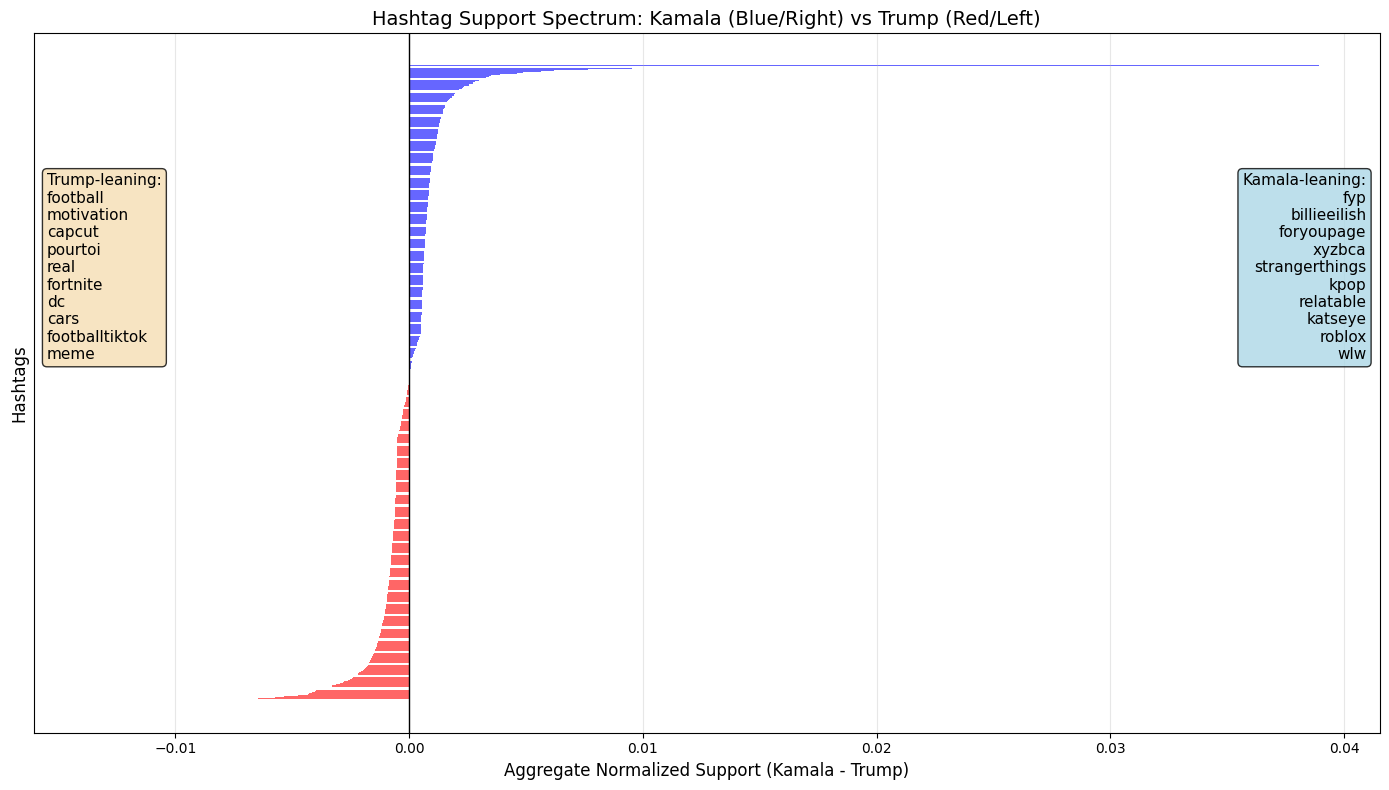
\includegraphics[width=\linewidth]{viz/hashtag_support.png}
        \captionsetup{width=0.9\linewidth, justification=centering} 
        \captionof{figure}{The distribution of differences between Harris corpus frequency and Trump corpus frequency for each hashtag.  Positive differences indicate higher normalized frequency in the corpus of Harris hashtags, whereas negative differences indicate higher normalized frequency in the corpus of Trump hashtags. The hashtags with the ten highest magnitude differences for each candidate's corpus are listed in the pale orange and pale blue boxes.}
        \label{hashtag_support}
    \end{minipage}
\end{adjustwidth}
\end{figure}

Notice also in Figure \ref{hashtag_support} that '\#fyp' is actually tagged at a higher frequency in Harris follower reposts than in Trump follower reposts; despite '\#fyp' having higher overall support in the Harris corpus, the frequent itemsets containing '\#fyp' have a tighter association in the Trump corpus. Other notable hashtags in the figure show which hashtags, while not occurring in the association rules, are more associated with which party. For example, '\#cars', '\#fortnite',\footnote{Fortnite is a popular video game} and '\#football' occur more frequently in Trump follower reposts, whereas '\#strangerthings',\footnote{\textit{Stranger Things} is a popular horror fiction television series set in the 1980s.} '\#kpop', and '\#wlw'\footnote{"WLW" is a common acronym for "women loving women."} occur more frequently in Harris follower reposts.

However, turning to Figure \ref{confidence_lift}, we see that the distribution of both confidence and lift of mined association rules is higher for Harris follower reposts than Trump follower reposts. The higher overall confidence suggests that the associations are more prevalent, while the higher overall lift connotes a unique association between consequent and antecedent. The implication is that on the whole, Harris followers have stronger and more consolidated association rules.

\begin{figure}[h]
\begin{adjustwidth}{-2cm}{-2cm}
    \begin{minipage}{\linewidth}
        \centering
        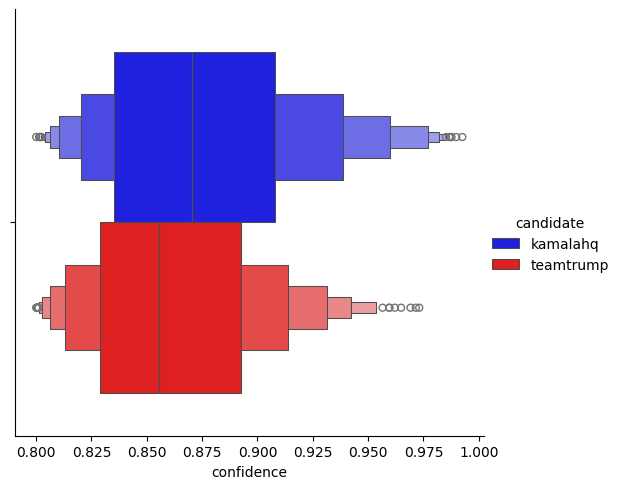
\includegraphics[width=0.5\linewidth]{viz/rule_confidence_dist.png}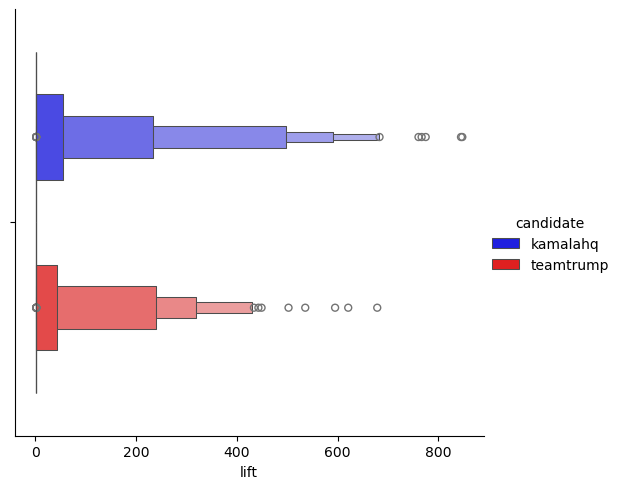
\includegraphics[width=0.5\linewidth]{viz/rule_lift_dist.png}
        \captionsetup{width=0.9\linewidth, justification=centering} 
        \captionof{figure}{Boxplots demonstrating the distribution of association rule confidence and association rule lift on the left and right, respectively.}
        \label{confidence_lift}
    \end{minipage}
\end{adjustwidth}
\end{figure}

\subsection{Hashtag Co-Occurrence Network Analysis}

\begin{figure}[h]
\begin{adjustwidth}{-2cm}{-2cm}
    \begin{minipage}{\linewidth}
        \centering
        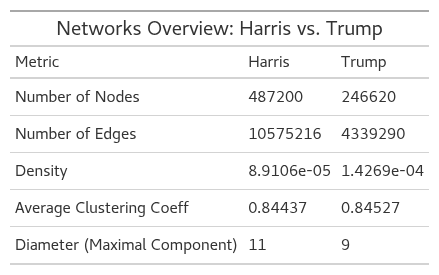
\includegraphics[width=0.5\linewidth]{viz/gt_network_stats.png}
        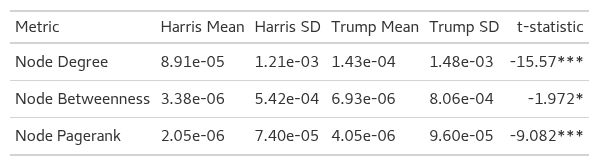
\includegraphics[width=0.7\linewidth]{viz/network_t_test.png}
        \captionsetup{width=0.9\linewidth, justification=centering} 
        \captionof{figure}{Network level descriptive statistics for the Harris and Trump hashtag co-occurrence social networks. Average Clustering Coefficient and Diameter are approximated with built-in networkx approximation algorithms, and the numbers shown here is an lower bound for the true value. Note that edges are weighted by the number of co-occurrences for any two hashtags. One TikTok repost equates to one co-occurrence. [I'll reformat the table and add my p values soon]}
        \label{network_stats}
    \end{minipage}
\end{adjustwidth}
\end{figure}

Pivoting now to the hashtag co-occurrence networks, we begin to find high-level structural patterns in the semantic discourse. A glance at Figure \ref{network_stats} shows that the the Harris network is larger, both in terms of nodes and edges as well as the diameter of the maximal component. This is in line with expectations, as there are more Harris follower reposts than Trump follower reposts. Interestingly,  despite the fact that Harris followers had higher average hashtags per repost, as shown in Section \ref{frequent_itemset_mining}, the Harris co-occurrence network has lower density. 

Figure \ref{network_stats} demonstrates that the Trump co-occurrence network, alongside being denser, has a higher average degree and higher average betweenness than the Harris co-occurrence network. This suggests that the semantic communities in the Trump co-occurrence network are more centrally concentrated and overlapping than those found in the Harris co-occurrence network.

As shown in Section \ref{frequent_itemset_mining}, engagement hacking hashtags appear frequently in both Harris and Trump follower reposts, and this is corroborated by the high centrality measures of engagement hacking hashtags in the co-occurrence networks. Notice in Figure \ref{high_centrality_nodes} that several of the high betweenness hashtags for both the Harris and Trump co-occurrence networks are not engagement hacking hashtags, but instead refer to substantively informative topics. One might conceptualize these substantive high betweenness hashtags as common and far-reaching topics that bridge disparate semantic communities. For the Trump co-occurrence network, those hashtags are '\#christmas', '\#history', and '\#sharinganeyes'.\footnote{The phrase "sharingan eyes" is a pop culture reference that originates from the Japanese manga and anime series \textit{Naruto}.} In the Harris co-occurrence network, these semantic bridges are '\#art' and '\#funny'.

While the two co-occurrence networks share similar average clustering coefficients and degree assortativity coefficient, the higher lift and confidence distribution for the Harris frequent itemsets in combination with a higher average node degree in the Trump co-occurrence network can provide an idea. These measures are consistent with Harris followers having more distinct, non-overlapping semantic communities and Trump followers having less distinct, overlapping semantic communities.

\begin{figure}[t]
\begin{adjustwidth}{-2cm}{-2cm}
    \begin{minipage}{\linewidth}
        \centering
        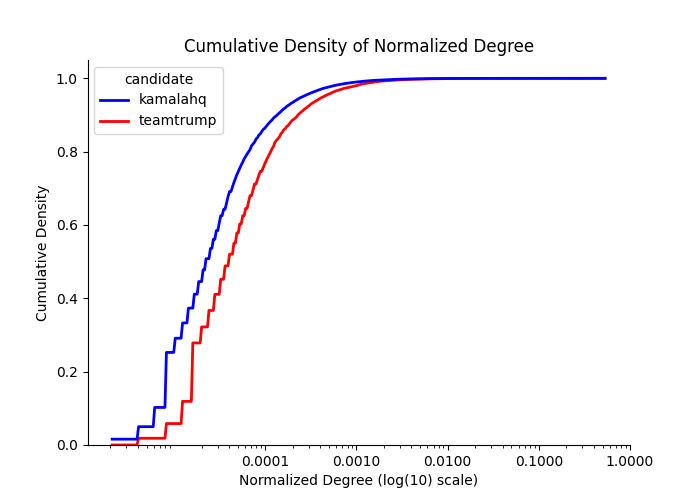
\includegraphics[width=0.7\linewidth]{viz/degree_density.png}
        \captionsetup{width=0.9\linewidth, justification=centering} 
        \captionof{figure}{Cumulative density graph for normalized node degree distributions of Harris and Trump co-occurrence networks.}
        \label{degree_density}
    \end{minipage}
\end{adjustwidth}
\end{figure}

\begin{figure}[t]
\begin{adjustwidth}{-2cm}{-2cm}
    \begin{minipage}{\linewidth}
        \centering
        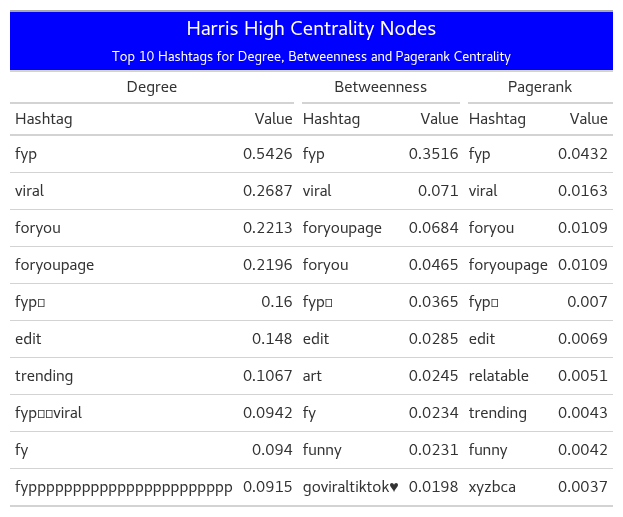
\includegraphics[height=0.4\textheight]{viz/kamala_high_centrality.png}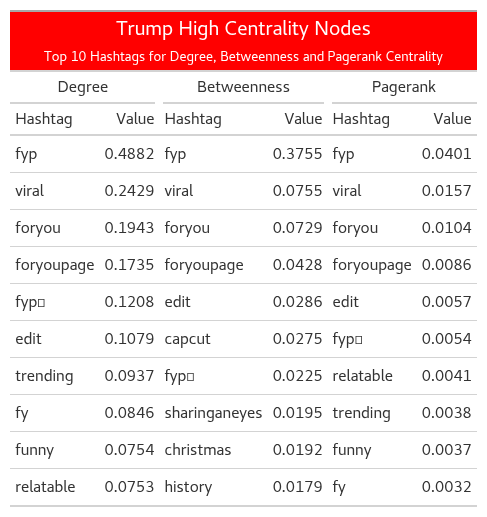
\includegraphics[height=0.4\textheight]{viz/trump_high_centrality.png}
        \captionsetup{width=0.9\linewidth, justification=centering} 
        \captionof{figure}{Hashtags with high centrality in the Harris and Trump co-occurrence networks displayed on the left and right, respectively.}
        \label{high_centrality_nodes}
    \end{minipage}
\end{adjustwidth}
\end{figure}

\subsection{BERTopic Bootstrap Models}


\begin{figure}[h]
\begin{adjustwidth}{-2cm}{-2cm}
    \begin{minipage}{\linewidth}
        \centering
        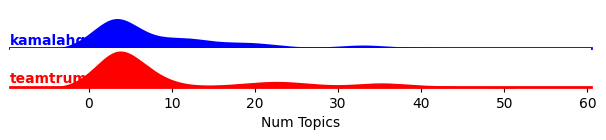
\includegraphics[width=0.5\linewidth]{viz/num_topics_dist.png}
        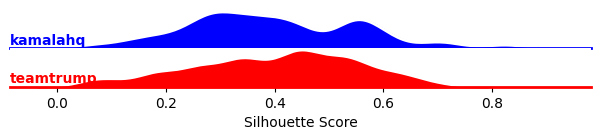
\includegraphics[width=0.5\linewidth]{viz/silhouette_score_dist.png}
        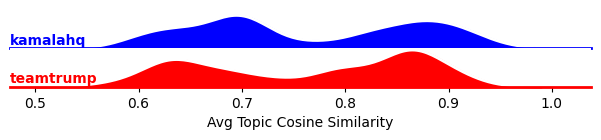
\includegraphics[width=0.5\linewidth]{viz/avg_cosine_similarity_dist.png}
        \captionsetup{width=0.9\linewidth, justification=centering} 
        \captionof{figure}{Distributions of various topic model measures across the 50 bootstrapped model iterations. Note that in BERTopic, topics are represented as vectors of \textit{n} dimension, where \textit{n} is the number of resulting dimensions from the dimension reduction model.}
        \label{bertopic_dists}
    \end{minipage}
\end{adjustwidth}
\end{figure}

\section{Discussion}

\subsection{Structure and Relation}

1) evidence that Trump has a more centralized and overlapping semantic landscape, and subsequently, Harris having a more concretized, distinct overlapping
2) consistency with previous literature

\subsection{Content Themes and Culture}

discuss some overarching themes:

gender and sexuality
sports and video games
music

distinguish between Harris having higher number of distinct, non-overlapping communities and Harris potentially having a more diverse semantic spread -- they're not the same thing! Trump and Harris corpora can be equally diverse in terms of the span of topics but may have different structural relations and distributions

with that being said, do examine semantic diversity, tell them what you find

\subsection{Culture Moderated by User Behaviors}

caveats in the data
1) trump users repost less; why?
2) billie eilish dominates; why?
3) non-representativeness and unknowable missingness

explain how this impacts the interpretation of the results

insofar as one accepts the results, explain what application or implication this knowledge has. is one group more susceptible to affective polarization? does rallying behind a candidate become more or less doable with the community strucutre?


\section{Conclusion}



%\lipsum[1-3]
\newpage

%\subsection*{Subtitle}
%\lipsum[4-5]
\nocite{*}

\section*{References}
\printbibliography[heading=none]
\end{document}